\documentclass[12pt]{charter}
\usepackage{enumerate}
\usepackage{graphicx}

% Definição da Página
\usepackage{changepage}
\usepackage{geometry}

\geometry{
    paper=a4paper, % Change to letterpaper for US letter
    inner=0.5cm, % Inner margin
    outer=0.8cm, % Outer margin
    bindingoffset=.5cm, % Binding offset
    top=1.5cm, % Top margin
    bottom=1.5cm, % Bottom margin
    marginpar=0.8cm,
   % showframe, % Uncomment to show how the type block is set on the page
}

% Diretório dos Gráficos
\graphicspath{ {./img/} }


\settitle{Cronograma do Projeto}{REEK Gaming}
\setauthor{Lenilson Dos Santos Silva}{ lenilsonspfc1@gmail.com }
\setstartdate
 %Dados da estrutura do Documento e pacotes necessários

\begin{document}
\maketitle
\thispagestyle{empty}
\newpage

\section*{Processo de definição da EEP - Especificação do Escopo do Projeto}
\label{sec:ciclovida}

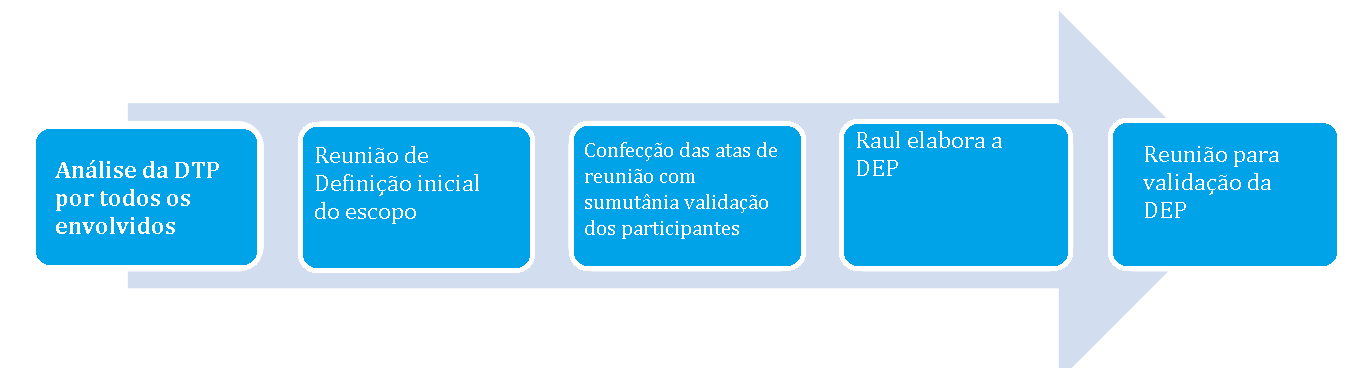
\includegraphics[scale=0.45]{img/PGE01.PNG}

\section*{Processos para criação, aprovação e manutenção da EAP}
\label{sec:ciclovida}

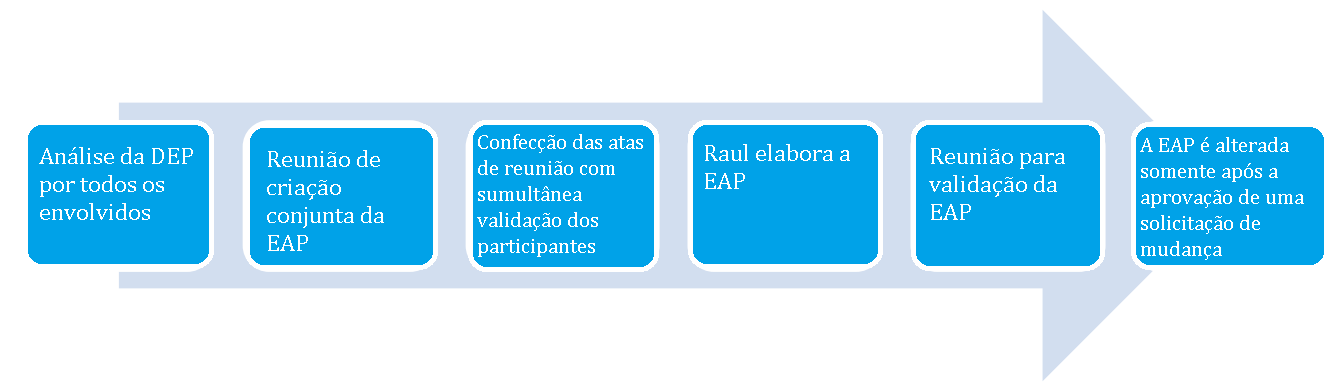
\includegraphics[scale=0.45]{img/PGE02.PNG}


\section*{Processos de aceitação das entregas}
\label{sec:ciclovida}

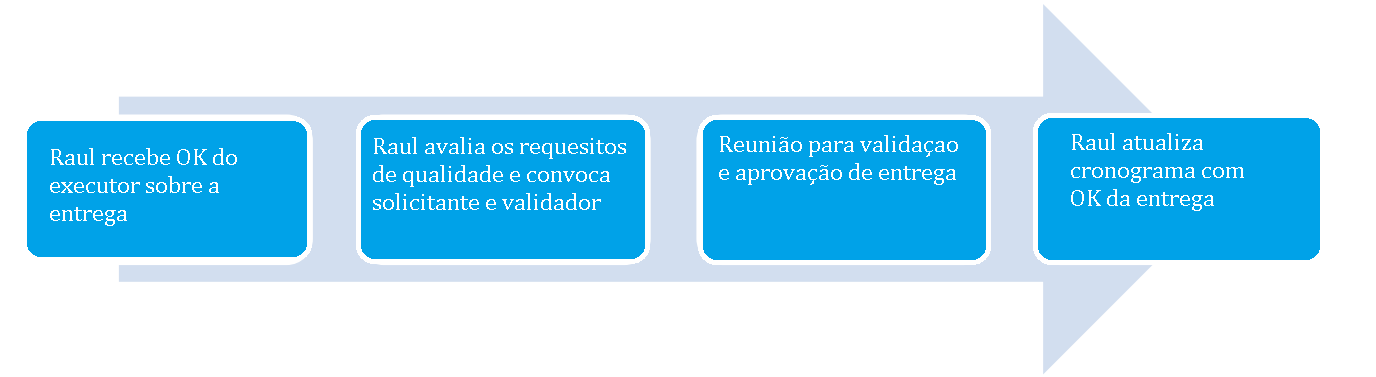
\includegraphics[scale=0.45]{img/PGE03.PNG}


\section*{Plano de gerenciamento de mudanças de escopo}
\label{sec:ciclovida}

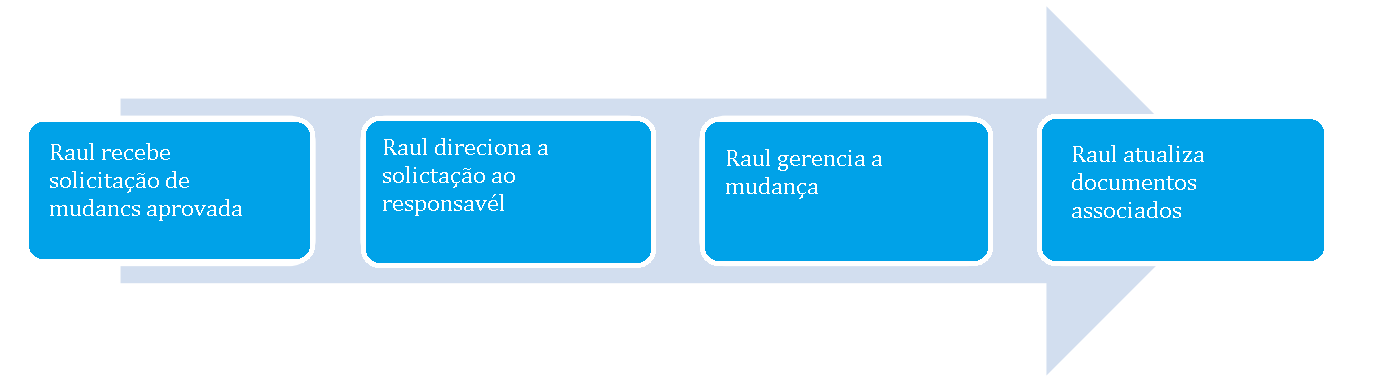
\includegraphics[scale=0.45]{img/PGE04.PNG}


\newline

\newline

\approvalsignature{Raul Donizeti}{Patrocinador / Gerente Projeto}

\approvalsignaturesecond{Lenilson Silva}{Patrocinador / Sub-Gerente Projeto}
\end{document}
